\documentclass[twoside]{book}

% Packages required by doxygen
\usepackage{fixltx2e}
\usepackage{calc}
\usepackage{doxygen}
\usepackage[export]{adjustbox} % also loads graphicx
\usepackage{graphicx}
\usepackage[utf8]{inputenc}
\usepackage{makeidx}
\usepackage{multicol}
\usepackage{multirow}
\PassOptionsToPackage{warn}{textcomp}
\usepackage{textcomp}
\usepackage[nointegrals]{wasysym}
\usepackage[table]{xcolor}

% Font selection
\usepackage[T1]{fontenc}
\usepackage[scaled=.90]{helvet}
\usepackage{courier}
\usepackage{amssymb}
\usepackage{sectsty}
\renewcommand{\familydefault}{\sfdefault}
\allsectionsfont{%
  \fontseries{bc}\selectfont%
  \color{darkgray}%
}
\renewcommand{\DoxyLabelFont}{%
  \fontseries{bc}\selectfont%
  \color{darkgray}%
}
\newcommand{\+}{\discretionary{\mbox{\scriptsize$\hookleftarrow$}}{}{}}

% Page & text layout
\usepackage{geometry}
\geometry{%
  a4paper,%
  top=2.5cm,%
  bottom=2.5cm,%
  left=2.5cm,%
  right=2.5cm%
}
\tolerance=750
\hfuzz=15pt
\hbadness=750
\setlength{\emergencystretch}{15pt}
\setlength{\parindent}{0cm}
\setlength{\parskip}{0.2cm}
\makeatletter
\renewcommand{\paragraph}{%
  \@startsection{paragraph}{4}{0ex}{-1.0ex}{1.0ex}{%
    \normalfont\normalsize\bfseries\SS@parafont%
  }%
}
\renewcommand{\subparagraph}{%
  \@startsection{subparagraph}{5}{0ex}{-1.0ex}{1.0ex}{%
    \normalfont\normalsize\bfseries\SS@subparafont%
  }%
}
\makeatother

% Headers & footers
\usepackage{fancyhdr}
\pagestyle{fancyplain}
\fancyhead[LE]{\fancyplain{}{\bfseries\thepage}}
\fancyhead[CE]{\fancyplain{}{}}
\fancyhead[RE]{\fancyplain{}{\bfseries\leftmark}}
\fancyhead[LO]{\fancyplain{}{\bfseries\rightmark}}
\fancyhead[CO]{\fancyplain{}{}}
\fancyhead[RO]{\fancyplain{}{\bfseries\thepage}}
\fancyfoot[LE]{\fancyplain{}{}}
\fancyfoot[CE]{\fancyplain{}{}}
\fancyfoot[RE]{\fancyplain{}{\bfseries\scriptsize Generated on Sun Nov 8 2015 14\+:07\+:33 for Prototype Design Pattern by Doxygen }}
\fancyfoot[LO]{\fancyplain{}{\bfseries\scriptsize Generated on Sun Nov 8 2015 14\+:07\+:33 for Prototype Design Pattern by Doxygen }}
\fancyfoot[CO]{\fancyplain{}{}}
\fancyfoot[RO]{\fancyplain{}{}}
\renewcommand{\footrulewidth}{0.4pt}
\renewcommand{\chaptermark}[1]{%
  \markboth{#1}{}%
}
\renewcommand{\sectionmark}[1]{%
  \markright{\thesection\ #1}%
}

% Indices & bibliography
\usepackage{natbib}
\usepackage[titles]{tocloft}
\setcounter{tocdepth}{3}
\setcounter{secnumdepth}{5}
\makeindex

% Hyperlinks (required, but should be loaded last)
\usepackage{ifpdf}
\ifpdf
  \usepackage[pdftex,pagebackref=true]{hyperref}
\else
  \usepackage[ps2pdf,pagebackref=true]{hyperref}
\fi
\hypersetup{%
  colorlinks=true,%
  linkcolor=blue,%
  citecolor=blue,%
  unicode%
}

% Custom commands
\newcommand{\clearemptydoublepage}{%
  \newpage{\pagestyle{empty}\cleardoublepage}%
}


%===== C O N T E N T S =====

\begin{document}

% Titlepage & ToC
\hypersetup{pageanchor=false,
             bookmarks=true,
             bookmarksnumbered=true,
             pdfencoding=unicode
            }
\pagenumbering{roman}
\begin{titlepage}
\vspace*{7cm}
\begin{center}%
{\Large Prototype Design Pattern }\\
\vspace*{1cm}
{\large Generated by Doxygen 1.8.10}\\
\vspace*{0.5cm}
{\small Sun Nov 8 2015 14:07:33}\\
\end{center}
\end{titlepage}
\clearemptydoublepage
\tableofcontents
\clearemptydoublepage
\pagenumbering{arabic}
\hypersetup{pageanchor=true}

%--- Begin generated contents ---
\chapter{Hierarchical Index}
\section{Class Hierarchy}
This inheritance list is sorted roughly, but not completely, alphabetically\+:\begin{DoxyCompactList}
\item \contentsline{section}{Ship}{\pageref{class_ship}}{}
\begin{DoxyCompactList}
\item \contentsline{section}{Patrol}{\pageref{class_patrol}}{}
\item \contentsline{section}{Submarine}{\pageref{class_submarine}}{}
\end{DoxyCompactList}
\item \contentsline{section}{Ship\+Manager}{\pageref{class_ship_manager}}{}
\end{DoxyCompactList}

\chapter{Class Index}
\section{Class List}
Here are the classes, structs, unions and interfaces with brief descriptions\+:\begin{DoxyCompactList}
\item\contentsline{section}{\hyperlink{class_patrol}{Patrol} }{\pageref{class_patrol}}{}
\item\contentsline{section}{\hyperlink{class_ship}{Ship} }{\pageref{class_ship}}{}
\item\contentsline{section}{\hyperlink{class_ship_manager}{Ship\+Manager} }{\pageref{class_ship_manager}}{}
\item\contentsline{section}{\hyperlink{class_submarine}{Submarine} }{\pageref{class_submarine}}{}
\end{DoxyCompactList}

\chapter{Class Documentation}
\hypertarget{class_patrol}{}\section{Patrol Class Reference}
\label{class_patrol}\index{Patrol@{Patrol}}
Inheritance diagram for Patrol\+:\begin{figure}[H]
\begin{center}
\leavevmode
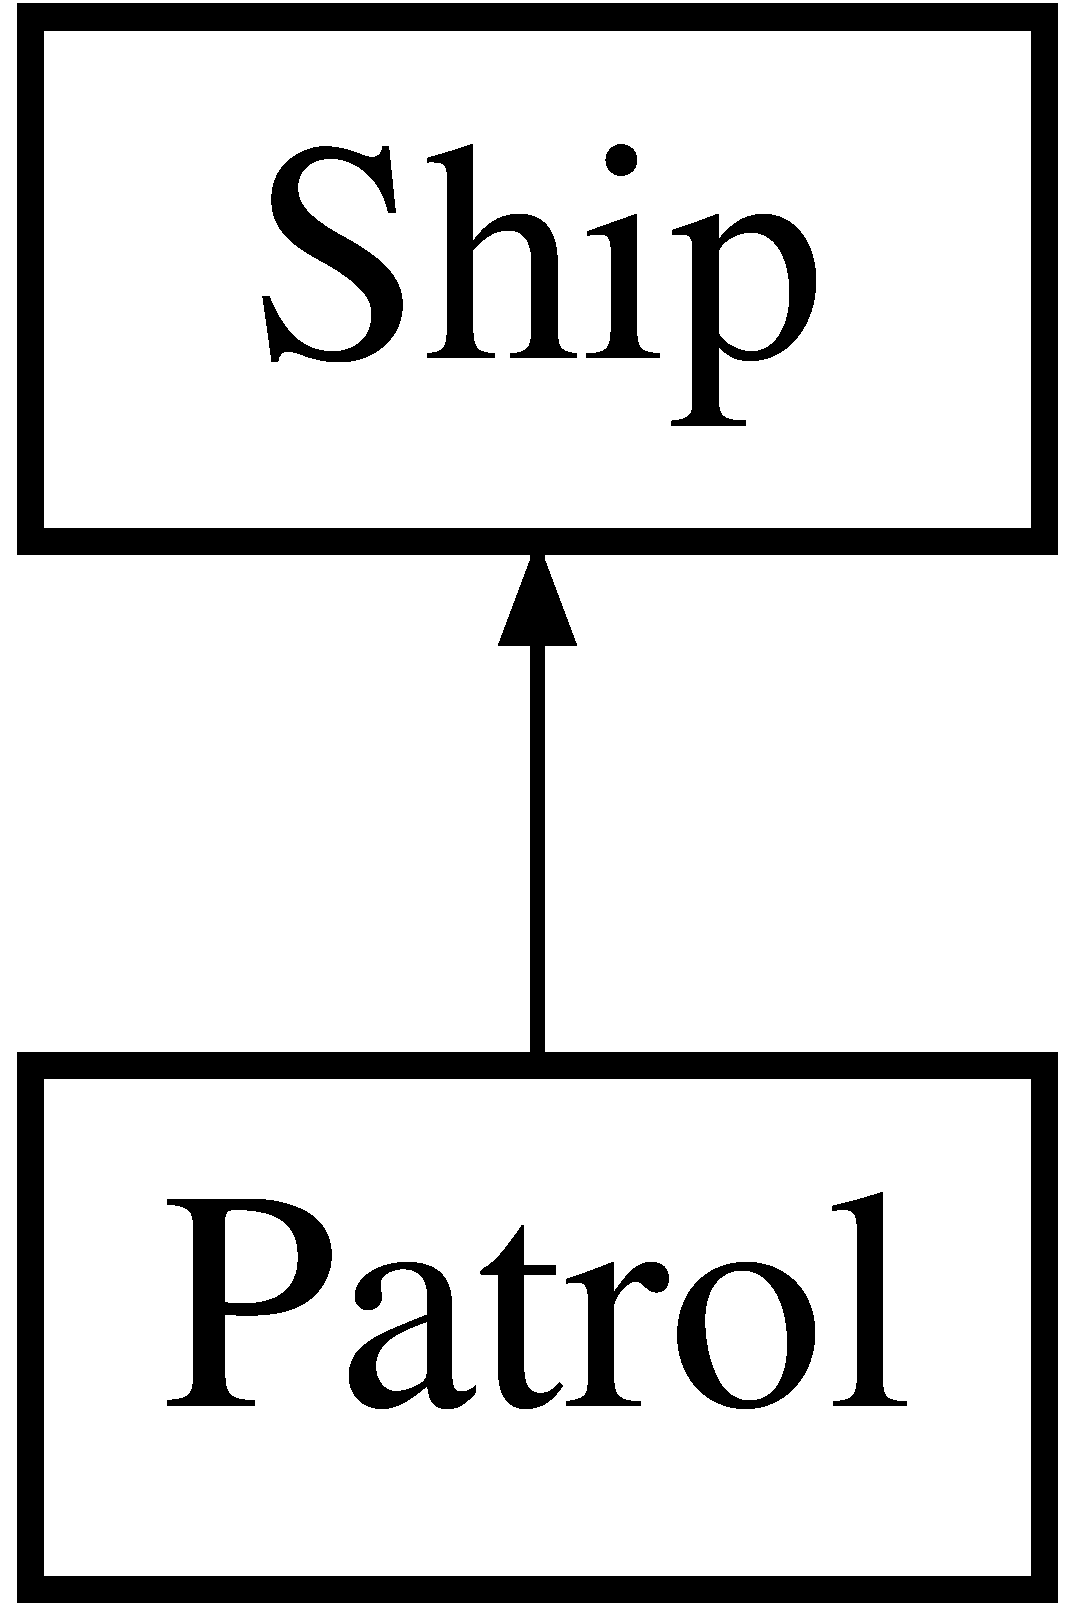
\includegraphics[height=2.000000cm]{class_patrol}
\end{center}
\end{figure}
\subsection*{Public Member Functions}
\begin{DoxyCompactItemize}
\item 
\hyperlink{class_patrol_a6c456b4e163008b4a5f15a01c31edb25}{Patrol} (std\+::string n, int h)
\item 
\hypertarget{class_patrol_a92289a0bace05e1e53e2bc41ba9b858a}{}\hyperlink{class_ship}{Ship} $\ast$ \hyperlink{class_patrol_a92289a0bace05e1e53e2bc41ba9b858a}{clone} ()\label{class_patrol_a92289a0bace05e1e53e2bc41ba9b858a}

\begin{DoxyCompactList}\small\item\em Create and return a pointer to a copy of this object. \end{DoxyCompactList}\end{DoxyCompactItemize}
\subsection*{Additional Inherited Members}


\subsection{Detailed Description}
A derived class of \hyperlink{class_ship}{Ship} representing a \hyperlink{class_patrol}{Patrol} 

\subsection{Constructor \& Destructor Documentation}
\hypertarget{class_patrol_a6c456b4e163008b4a5f15a01c31edb25}{}\index{Patrol@{Patrol}!Patrol@{Patrol}}
\index{Patrol@{Patrol}!Patrol@{Patrol}}
\subsubsection[{Patrol(std\+::string n, int h)}]{\setlength{\rightskip}{0pt plus 5cm}Patrol\+::\+Patrol (
\begin{DoxyParamCaption}
\item[{std\+::string}]{n, }
\item[{int}]{h}
\end{DoxyParamCaption}
)\hspace{0.3cm}{\ttfamily [inline]}}\label{class_patrol_a6c456b4e163008b4a5f15a01c31edb25}
Constructs a \hyperlink{class_patrol}{Patrol} with the specified name and health. 

The documentation for this class was generated from the following file\+:\begin{DoxyCompactItemize}
\item 
Seng330\+A2.\+cpp\end{DoxyCompactItemize}

\hypertarget{class_ship}{}\section{Ship Class Reference}
\label{class_ship}\index{Ship@{Ship}}
Inheritance diagram for Ship\+:\begin{figure}[H]
\begin{center}
\leavevmode
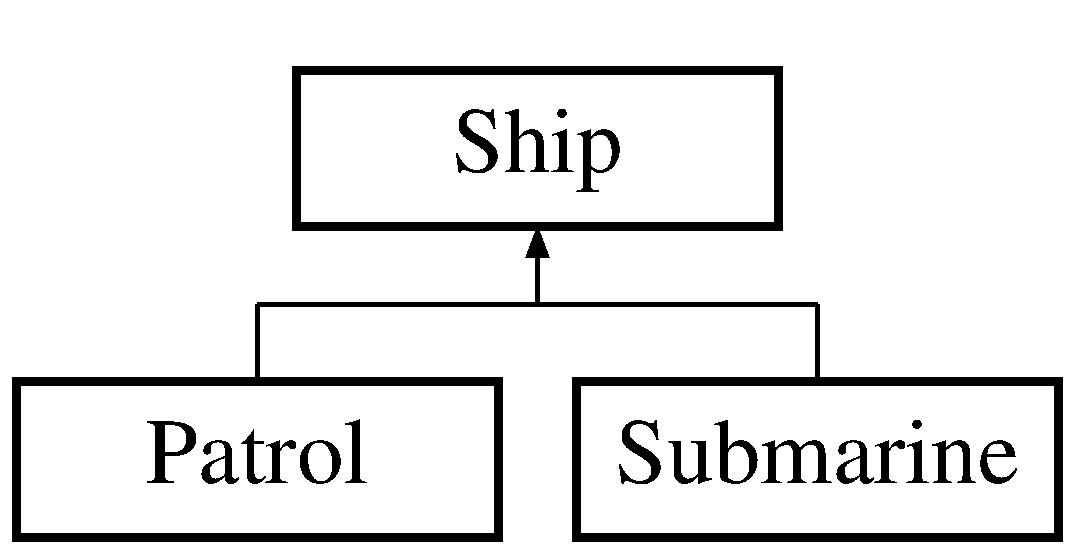
\includegraphics[height=2.000000cm]{class_ship}
\end{center}
\end{figure}
\subsection*{Public Member Functions}
\begin{DoxyCompactItemize}
\item 
\hypertarget{class_ship_a929dfa0b467a100d7a9ad52f8a29ef94}{}virtual \hyperlink{class_ship}{Ship} $\ast$ \hyperlink{class_ship_a929dfa0b467a100d7a9ad52f8a29ef94}{clone} ()=0\label{class_ship_a929dfa0b467a100d7a9ad52f8a29ef94}

\begin{DoxyCompactList}\small\item\em Create and return a pointer to a copy of this object. \end{DoxyCompactList}\item 
\hypertarget{class_ship_ad9907b498c9d7f2f0c62fabbc5ab050b}{}std\+::string \hyperlink{class_ship_ad9907b498c9d7f2f0c62fabbc5ab050b}{get\+Name} ()\label{class_ship_ad9907b498c9d7f2f0c62fabbc5ab050b}

\begin{DoxyCompactList}\small\item\em Returns the name of the ship. \end{DoxyCompactList}\item 
\hypertarget{class_ship_afc4fca85c159457aeac07a9f1c21d06e}{}int \hyperlink{class_ship_afc4fca85c159457aeac07a9f1c21d06e}{get\+Health} ()\label{class_ship_afc4fca85c159457aeac07a9f1c21d06e}

\begin{DoxyCompactList}\small\item\em Returns the health of the ship. \end{DoxyCompactList}\end{DoxyCompactItemize}
\subsection*{Protected Attributes}
\begin{DoxyCompactItemize}
\item 
\hypertarget{class_ship_a110781c5f23a8c9a9cfc010601ea32b8}{}int \hyperlink{class_ship_a110781c5f23a8c9a9cfc010601ea32b8}{health}\label{class_ship_a110781c5f23a8c9a9cfc010601ea32b8}

\begin{DoxyCompactList}\small\item\em The health of the ship. \end{DoxyCompactList}\item 
\hypertarget{class_ship_a2e1ec44d8edcfc20d8d580f95fd6af75}{}std\+::string \hyperlink{class_ship_a2e1ec44d8edcfc20d8d580f95fd6af75}{name}\label{class_ship_a2e1ec44d8edcfc20d8d580f95fd6af75}

\begin{DoxyCompactList}\small\item\em The name of the ship. \end{DoxyCompactList}\end{DoxyCompactItemize}


The documentation for this class was generated from the following files\+:\begin{DoxyCompactItemize}
\item 
src/Ship.\+h\item 
src/Ship.\+cpp\end{DoxyCompactItemize}

\hypertarget{class_ship_manager}{}\section{Ship\+Manager Class Reference}
\label{class_ship_manager}\index{Ship\+Manager@{Ship\+Manager}}
\subsection*{Static Public Member Functions}
\begin{DoxyCompactItemize}
\item 
static \hyperlink{class_ship}{Ship} $\ast$ \hyperlink{class_ship_manager_a723e98f2f7938f7c4f6f293d9a9bf71b}{get\+Patrol} ()
\item 
static \hyperlink{class_ship}{Ship} $\ast$ \hyperlink{class_ship_manager_a69da6e8e716dde8e9f077beefd5a9863}{get\+Submarine} ()
\end{DoxyCompactItemize}


\subsection{Detailed Description}
A static class that creates \hyperlink{class_ship}{Ship} objects on demand 

\subsection{Member Function Documentation}
\hypertarget{class_ship_manager_a723e98f2f7938f7c4f6f293d9a9bf71b}{}\index{Ship\+Manager@{Ship\+Manager}!get\+Patrol@{get\+Patrol}}
\index{get\+Patrol@{get\+Patrol}!Ship\+Manager@{Ship\+Manager}}
\subsubsection[{get\+Patrol()}]{\setlength{\rightskip}{0pt plus 5cm}static {\bf Ship}$\ast$ Ship\+Manager\+::get\+Patrol (
\begin{DoxyParamCaption}
{}
\end{DoxyParamCaption}
)\hspace{0.3cm}{\ttfamily [inline]}, {\ttfamily [static]}}\label{class_ship_manager_a723e98f2f7938f7c4f6f293d9a9bf71b}
Clone and return a pointer to a copy of its \hyperlink{class_patrol}{Patrol} object prototype \hypertarget{class_ship_manager_a69da6e8e716dde8e9f077beefd5a9863}{}\index{Ship\+Manager@{Ship\+Manager}!get\+Submarine@{get\+Submarine}}
\index{get\+Submarine@{get\+Submarine}!Ship\+Manager@{Ship\+Manager}}
\subsubsection[{get\+Submarine()}]{\setlength{\rightskip}{0pt plus 5cm}static {\bf Ship}$\ast$ Ship\+Manager\+::get\+Submarine (
\begin{DoxyParamCaption}
{}
\end{DoxyParamCaption}
)\hspace{0.3cm}{\ttfamily [inline]}, {\ttfamily [static]}}\label{class_ship_manager_a69da6e8e716dde8e9f077beefd5a9863}
Clone and return a pointer to a copy of its \hyperlink{class_submarine}{Submarine} object prototype 

The documentation for this class was generated from the following file\+:\begin{DoxyCompactItemize}
\item 
Seng330\+A2.\+cpp\end{DoxyCompactItemize}

\hypertarget{class_submarine}{}\section{Submarine Class Reference}
\label{class_submarine}\index{Submarine@{Submarine}}


{\ttfamily \#include $<$Submarine.\+h$>$}

Inheritance diagram for Submarine\+:\begin{figure}[H]
\begin{center}
\leavevmode
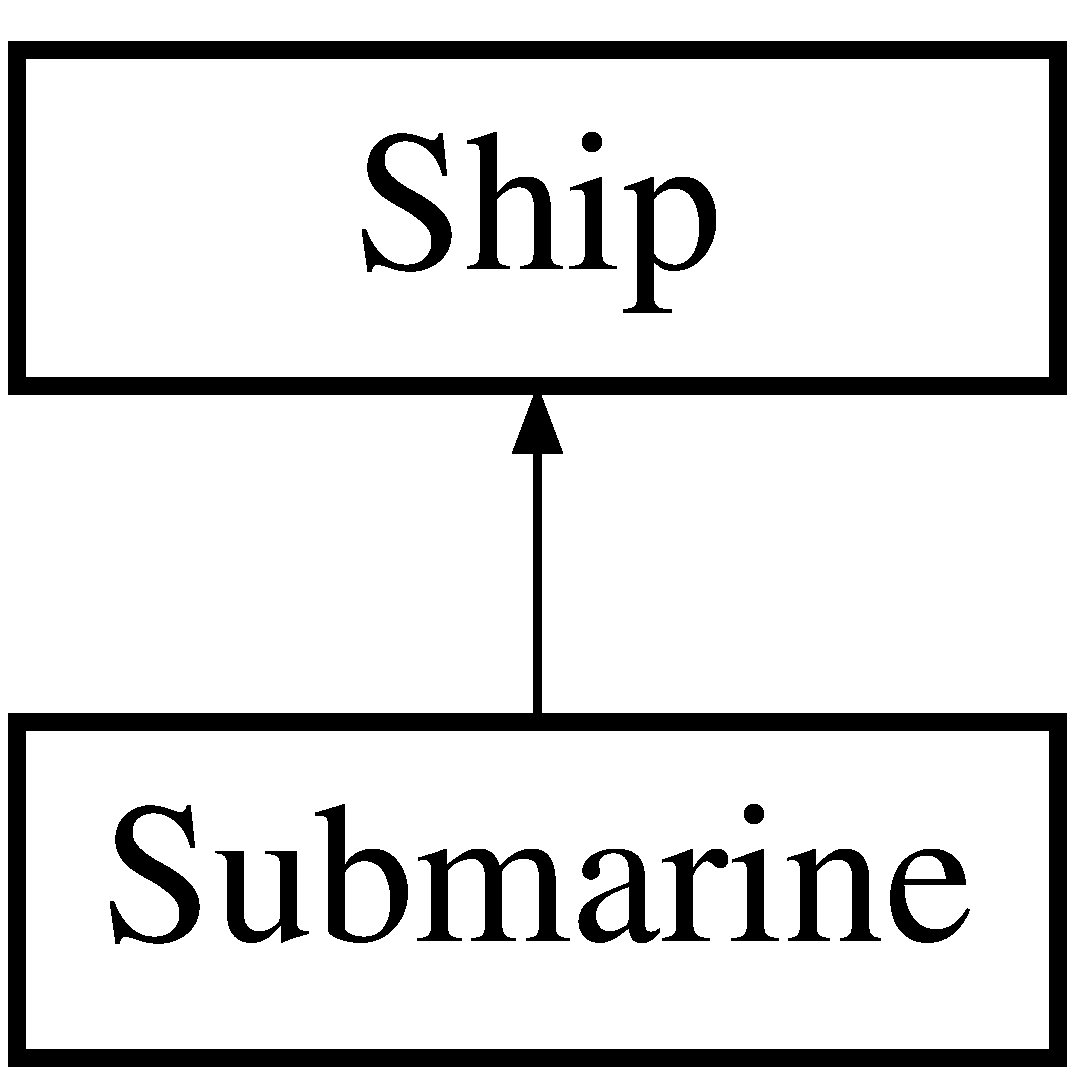
\includegraphics[height=2.000000cm]{class_submarine}
\end{center}
\end{figure}
\subsection*{Public Member Functions}
\begin{DoxyCompactItemize}
\item 
\hyperlink{class_submarine_ac59d1fd118990f8173121e27926a1ce0}{Submarine} (std\+::string n, int h)
\item 
\hypertarget{class_submarine_a1affdf9e8e3f14ddf2d2ea04157506b2}{}\hyperlink{class_ship}{Ship} $\ast$ \hyperlink{class_submarine_a1affdf9e8e3f14ddf2d2ea04157506b2}{clone} ()\label{class_submarine_a1affdf9e8e3f14ddf2d2ea04157506b2}

\begin{DoxyCompactList}\small\item\em Create and return a pointer to a copy of this object. \end{DoxyCompactList}\end{DoxyCompactItemize}
\subsection*{Additional Inherited Members}


\subsection{Detailed Description}
A derived class of \hyperlink{class_ship}{Ship} representing a \hyperlink{class_submarine}{Submarine} 

\subsection{Constructor \& Destructor Documentation}
\hypertarget{class_submarine_ac59d1fd118990f8173121e27926a1ce0}{}\index{Submarine@{Submarine}!Submarine@{Submarine}}
\index{Submarine@{Submarine}!Submarine@{Submarine}}
\subsubsection[{Submarine(std\+::string n, int h)}]{\setlength{\rightskip}{0pt plus 5cm}Submarine\+::\+Submarine (
\begin{DoxyParamCaption}
\item[{std\+::string}]{n, }
\item[{int}]{h}
\end{DoxyParamCaption}
)}\label{class_submarine_ac59d1fd118990f8173121e27926a1ce0}
Constructs a \hyperlink{class_submarine}{Submarine} with the specified name and health. 

The documentation for this class was generated from the following files\+:\begin{DoxyCompactItemize}
\item 
src/Submarine.\+h\item 
src/Submarine.\+cpp\end{DoxyCompactItemize}

%--- End generated contents ---

% Index
\backmatter
\newpage
\phantomsection
\clearemptydoublepage
\addcontentsline{toc}{chapter}{Index}
\printindex

\end{document}
